\chapter{Dispersion relation}
\label{disperrel}
A dispersion relation relates the wavenumber of a wave to its frequency. We
will see that this relation is of utmost importance when discussing periodic
lattices as only waves of certain frequencies are transmitted by the lattice.

\section{1d lattice}
\begin{figure}[!h]
\begin{center}
  \begin{tikzpicture}
  {[start chain,every on chain/.style=join,every join/.style=-,
    state/.style={circle,draw,minimum size=1.5cm}]
     \node[on chain] (A) {$\cdots$};
     \node[on chain,state] (B) {$M_{n-1}$};
     \node[on chain,state] (C) {$M_n$};
     \node[on chain,state] (D) {$M_{n+1}$};
     \node[on chain] (E) {$\cdots$};
  }
  \end{tikzpicture}
  \caption{\label{fig:sqscheme1d} Schematic view of our 1d model.}
\end{center}
\end{figure}

Let us start our discussion with the most basic one-dimensional case. In this
case, we have masses of equal mass, $m$ spread out evenly across one dimension.
All neighbouring masses are connected by an elastic force which scales
proportionally with distance, i.e. $F = kx$ for some $k$.

% TODO: Add discussion about transverse waves into appendix?
\textit{Note}: As mentioned before, we will be thinking of this system as a
mass-spring system. Notice however that it does not matter whether we are
considering longitudinal or transverse waves, as the equations governing their
interactions are the same. In our discussions, we will be considering the waves
propagating through our models as transverse waves. This helps to simplify
visualisations as the displacements and movements of the masses are
perpendicular to the lattice on which they are bound.

With this one-dimensional case set up, we now want to find out what forms of
waves it allows to propagate. We do this by considering only nearest neighbour
interactions and examining the elementary unit of the lattice which can be
repeated by translation to form the full lattice.

So let us consider three masses side-by-side in our lattice, $M_{n-1}$, $M_n$
and $M_{n+1}$ which are $y_{n-1}$, $y_n$ and $y_{n+1}$ displacement away from
their equilibrium positions. By focusing on the centre mass and considering
only nearest neighbour interactions, by Hooke's Law, we have that the force on
$M_n$

\begin{align}
  F_{n}=\sum F=k\left(y_{n-1}+y_{n+1}-2y_{n}\right) \label{eq:HL}
\end{align}

At the same time, we have by Newton's 2nd Law that

\begin{align}
  F_{n}=m\frac{d^{2}}{dt^{2}}y_{n}
\end{align}

Taking $y_n$ to be the general wave solution

\begin{align}
  &y_{n}=\hat{y}_{n}e^{-i\Omega t} \\
  \Rightarrow &\frac{d^{2}}{dt^{2}}y_{n}=-\Omega^{2}y_{n} \\
  \Rightarrow &F_{n}=-m\Omega^{2}y_{n} \label{eq:N2L}
\end{align}

where $\Omega$ is the frequency of the wave and $\hat{y}_{n}$ is the complex
amplitude.

Therefore, we have by \eqref{eq:HL} and \eqref{eq:N2L} that

\begin{align}
  &-m\Omega^{2}y_{n}=k\left(y_{n-1}+y_{n+1}-2y_{n}\right) \\
  \Rightarrow &\left(-\frac{m}{k}\Omega^{2}+2\right)y_{n}-y_{n-1}-y_{n+1}=0
    \label{eq:HLN2L}
\end{align}

Since we can write this differential equation for any of our masses in our
infinite lattice, we would need to solve an infinite number of coupled second
order differential equations. However, the trick we use is that since we have
that $M_{n-1}$ and $M_{n+1}$ are equidistant from $M_{n}$ at equilibrium (i.e.
the lattice is periodic), we can make use of Bloch's theorem\cite{bloch} to
describe the phase shift in the wave solution as

\begin{align}
  y_{n-1}=e^{-i\kappa}y_n,\ \ y_{n+1}=e^{i\kappa}y_n
\end{align}

Hence, from \eqref{eq:HLN2L}, we see that

\begin{align}
  &\left(-\frac{m}{k}\Omega^{2}+2-e^{-i\kappa}-e^{i\kappa}\right)y_{n}=0 \\
  \Rightarrow &\cos\left(\kappa\right)=-\frac{m}{2k}\Omega^{2}+1
\end{align}

Therefore, we now have an equation linking the wave number $\kappa$ and the
frequency $\Omega$ of waves propagating across our 1d lattice. By initialising
$m$ and $k$ we can use this equation to plot the dispersion curve of our
system. By setting $m=k=1$, we get the dispersion curve in Figure
~\ref{fig:dc1}.

\begin{figure}[!h]
\centering
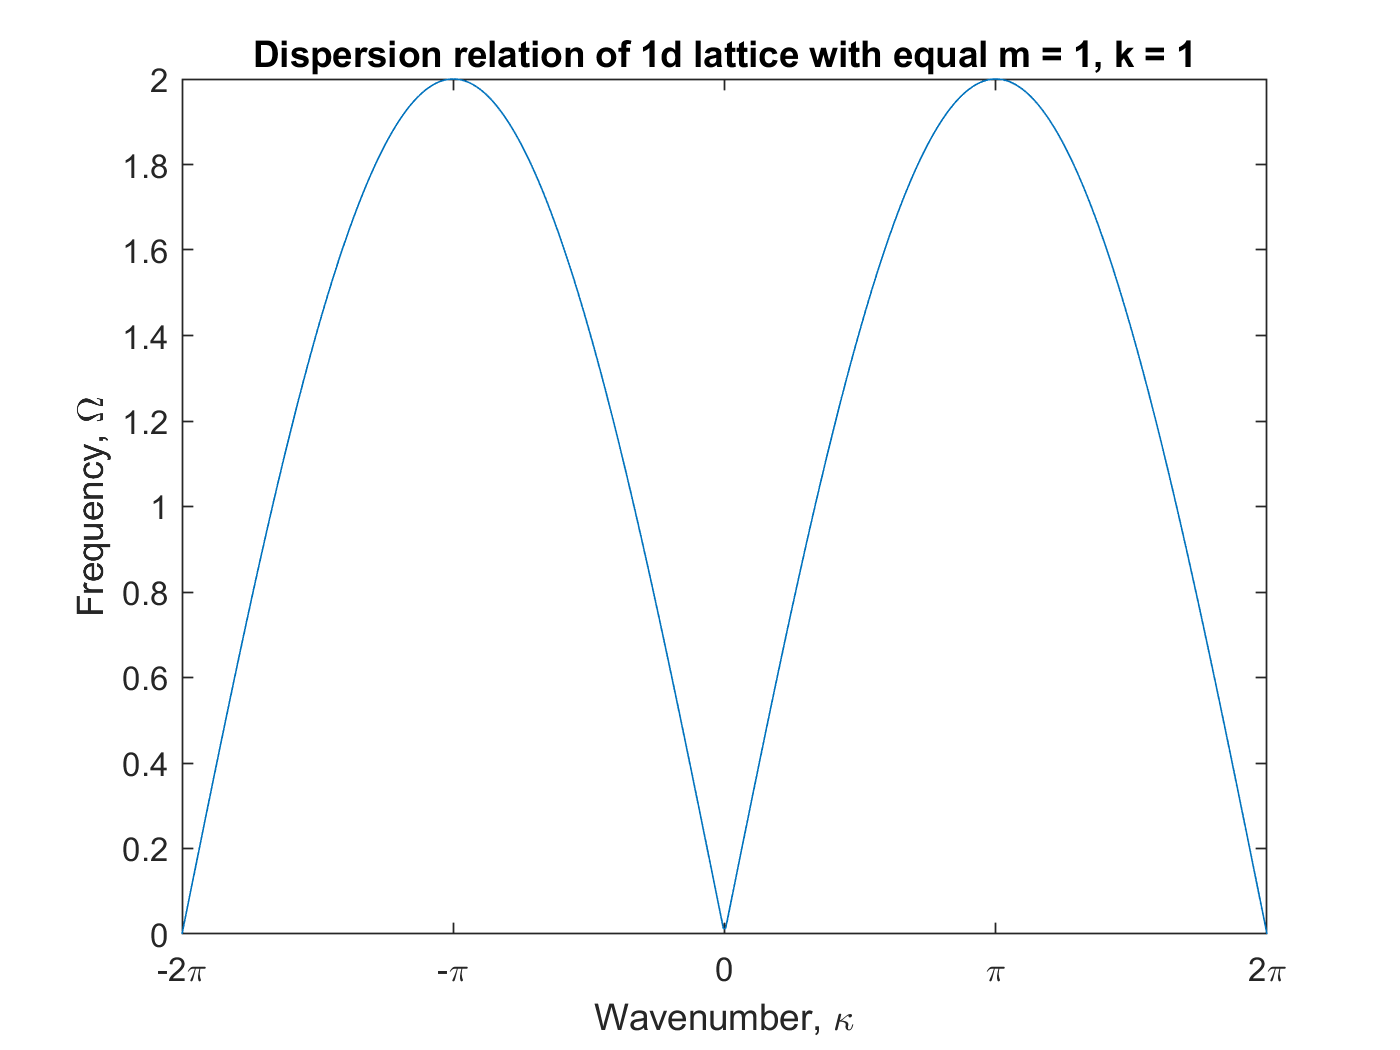
\includegraphics[width=0.8\textwidth]{imgs/1ddispersion.png}
\caption{\label{fig:dc1}Dispersion relation of a 1d monoatomic
         chain.}
\end{figure}

The first interesting thing to notice about this dispersion relation is that
the curve seems to be periodically repeating. More precisely, if we look at the
curve between $-\pi$ and $\pi$, we can see that translating this portion of the
graph left or right by $2\pi$ will give us the rest of the dispersion relation.
This range of wave numbers is known as the first Brillouin zone, which we will
discuss more in the context of 2d lattices in Chapter \ref{brizones}.

\section{2d square lattice}
\begin{figure}[!h]
\centering
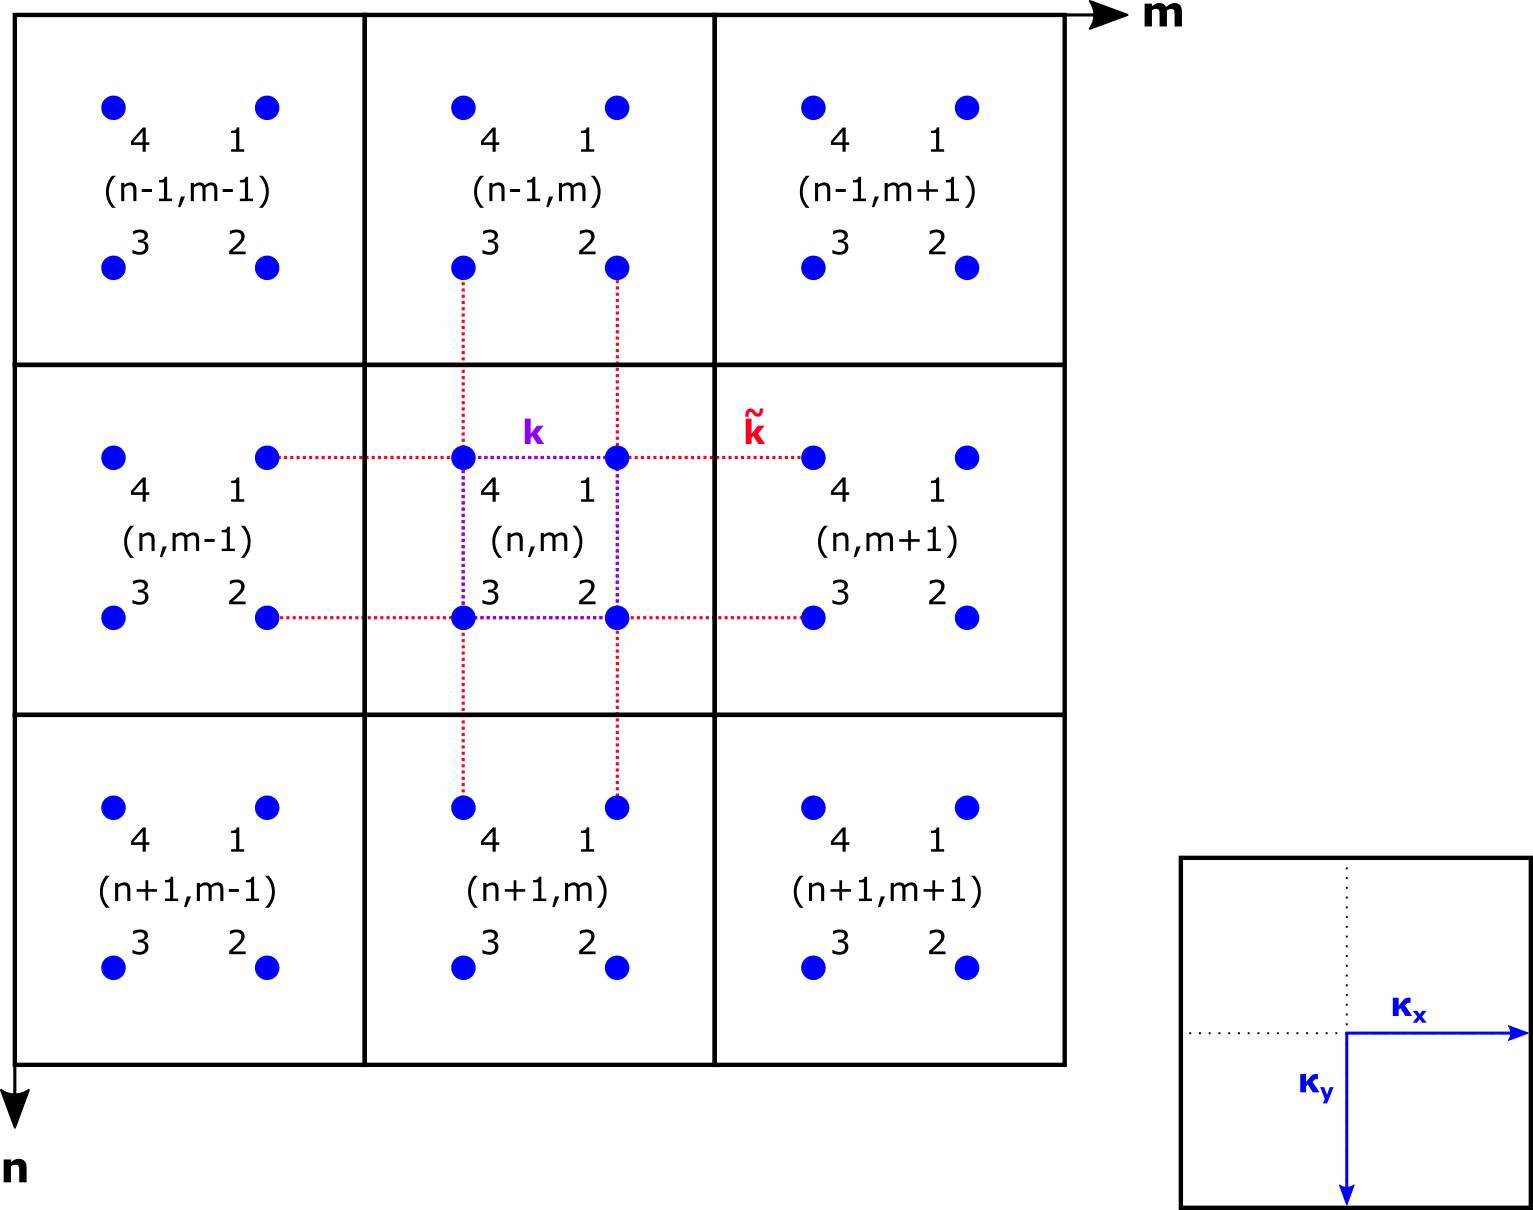
\includegraphics[width=0.8\textwidth]{imgs/sqmodel.png}
\caption{\label{fig:sqscheme} Schematic view of our 2d model. Each square
  tile in the grid corresponds to one elementary cell with four masses. $k$ and
  $\tilde{k}$ represent the intra- and inter-cell spring constants
  respectively. The cell in the far bottom right shows the directions of the
  Bloch phases. Note that only the elastic interactions involving the masses in
  cell $(n,m)$ are shown to avoid cluttering the figure, although they exist
  within and between each cell.}
\end{figure}

We now extend this analysis to an infinite two-dimensional square lattice, as
described in Figure~\ref{fig:sqscheme}. Each elementary square cell contains
four masses $M_i$ for $i\in\left[1, 4\right]$ which are arranged clockwise from
the top right. We take $n$ and $m$ to be the vertical and horizontal directions
respectively, with $n$ increasing downwards and $m$ increasing to the right, so
that relative to cell $(n, m)$ we have cell $(n-1,m)$ above and cell $(n,m+1)$
to the right. We have decided to go with this convention as it reflects matrix
indexing in Matlab, which will simplify our code. With this setup, we can now
label each mass and its displacement uniquely, e.g. $M_i$ in cell $(n, m)$ is
labelled $M_i^{n,m}$ and has displacement $y_i^{n,m}$.

\textit{Note:} Though we use this system to refer to specific masses in
specific cells, the mass of each mass is determined solely by its position in
its cell, i.e. $\forall n,m\in\mathbb{Z}$, the mass of $M_i^{n,m}=M_i$.

Each mass is elastically connected to its direct neighbours, e.g. $M_1^{n,m}$
is connected to $M_2^{n,m}$, $M_4^{n,m}$, $M_2^{n-1,m}$ and $M_4^{n,m+1}$. We
have the spring constant $k$ between masses in the same cell and $\tilde{k}$
between masses in adjacent cells.

Now again we consider only nearest neighbour interactions. Focusing on the
elementary cell $(n,m)$ and its adjacent cells, using Hooke's law and Newton's
2nd law on each of the masses in cell $(n,m)$, we can get a second order
differential equation which is coupled to the displacements of the other masses
it is connected to. For example, considering $M_1^{n,m}$, we get

\begin{align}
  F_1=M_1\frac{d^{2}}{dt^{2}}y_1^{n,m}
      =k\left(y_2^{n,m}+y_4^{n,m}-2y_1^{n,m}\right)+
       \tilde{k}\left(y_2^{n-1,m}+y_4^{n,m+1}-2y_1^{n,m}\right)
\label{eq:2dM1}
\end{align}

Since we can write this differential equation for any of our masses in our
infinite lattice, we would get an infinite number of coupled second order
differential equation. However, similar to the 1d case, using the periodicity
of the lattice and Bloch's theorem once more, we can relate the displacements
of each mass to the corresponding mass in a \textit{base cell} with the lattice
vectors $\kappa_y$ and $\kappa_x$, i.e.

\begin{align}
  y_i^{n+N,m+M}=e^{i\left(N\kappa_y+M\kappa_x\right)}y_i^{n,m}\ \ \ \ 
      \forall N,M\in\mathbb{Z}
\end{align}

With this, instead of an infinite number of equations, we have a set of four
coupled second order differential equations, one for each $y_i^{n,m}$ for
$i\in\left[1,4\right]$. We now drop the superscripts $\left(n,m\right)$ and
assume we have a wave solution of the form  

\begin{align}
  &y_{i}=\hat{y}_{i}e^{-i\Omega t} \\
  \Rightarrow &\frac{d^{2}}{dt^{2}}y_{i}=-\Omega^{2}y_{i} \\
  \Rightarrow &F_{i}=-M_i\Omega_i^{2}y_{i}
\label{eq:wavesol}
\end{align}

where $\Omega$ is the frequency of the wave and $\hat{y}_{n}$ is the complex
amplitude. We can now rewrite \eqref{eq:2dM1} as

\begin{align}
  M_1\Omega_1^{2}y_1
      &=k\left(2y_1-y_2-y_4\right)+
       \tilde{k}\left(2y_1-y_{2}e^{-i\kappa_y}-y_{4}e^{i\kappa_x}\right) \\
      &=\left(2k+2\tilde{k}\right)y_1+\left(-k-\tilde{k}e^{-i\kappa_y}\right)y_2+
       \left(-k-\tilde{k}e^{i\kappa_x}\right)y_4
\end{align}

By constructing this equation for each $y_i$, we can reformulate these four
difference equations as an eigenvalue problem

\begin{align}
  \left[\matr{A}\left(\kappa_{x},\kappa_{y}\right)-\matr{\Omega}\matr{M}\right]\vec{y}=\vec{0}
\label{eq:sqeig}
\end{align}

where $\matr{\Omega}=\diag\left(\left\{\Omega_i^2\right\}\right)$,
$\matr{M}=\diag\left(\left\{M_i\right\}\right)$,
$\vec{y}=\left[\left\{y_i\right\}\right]^T$ and

\begin{align}
  \matr{A}\left(\kappa_{x},\kappa_{y}\right)=\left[
\begin{array}{cccc}
2k+\tilde{k} & -k-\tilde{k}e^{-i\kappa_{y}} & 0 & -k-\tilde{k}e^{i\kappa_{x}}\\
-k-\tilde{k}e^{i\kappa_{y}} & 2k+\tilde{\tilde{k}} & -k-\tilde{k}e^{i\kappa_{x}} & 0\\
0 & -k-\tilde{k}e^{-i\kappa_{x}} & 2k+\tilde{\tilde{k}} & -k-\tilde{k}e^{i\kappa_{y}}\\
-k-\tilde{k}e^{-i\kappa_{x}} & 0 & -k-\tilde{k}e^{-i\kappa_{y}} & 2k+\tilde{\tilde{k}}
\end{array}\right]
\end{align}

Therefore, we can solve for the eigenvalues and eigenvectors of this equation.
The eigenvalues of this equation correspond to the frequency of waves,
$\Omega$, which are allowed through our lattice while the eigenvectors
correspond to the displacement of the masses, $y_i$. However, the next question
arises: How should we vary $\kappa$ so that we get a good enough picture of the
full dispersion relation of our 2d lattice?

To answer this question, we first have to discuss the theory of Brillouin zones.

\subsection{Brillouin zones}
\label{brizones}
%TODO: Molding the flow of light might be useful
The concept of Brillouin zones was first defined by Leon Brillouin in his book
on wave propagation in periodic structures.\cite{brillouin} The Brillouin zone
is a particular choice of the unit cell of the reciprocal lattice, where a
reciprocal lattice represents the Fourier transform of another lattice. In our
case, our model lattice is a periodic spatial function in real space, and so
its reciprocal lattice exists as a function of frequency in reciprocal space.

As we are able to tessellate our physical lattice with a periodically repeating
unit cell, so there exists a unit reciprocal cell which can cover the
reciprocal space without overlap. A Brillouin zone is a particular choice of
this reciprocal cell and is constructed as the set of points enclosed by the
Bragg planes. The Bragg planes exist in reciprocal space and are the planes
perpendicular to a straight line from the origin to each lattice point. These
concepts are described visually for a 2d square real lattice in
Figure~\ref{fig:bzonesq}.

\begin{figure}[!h]
\centering
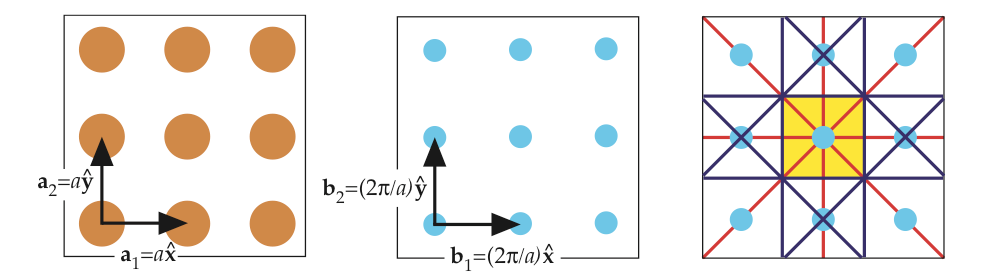
\includegraphics[width=0.8\textwidth]{imgs/bzonesq.png}
\caption{\label{fig:bzonesq} On the left is the lattice points in real space.
    In the middle is the corresponding reciprocal lattice. On the right is the
    construction of the first Brillouin zone: straight lines are drawn from the
    origin to the other lattice points (red), their perpendicular bisectors are
    the Bragg planes (blue), and the innermost region enclosed by the Bragg
    planes is the first Brilloin zone (yellow). Image and caption adapted from
    source.\cite{MITnp}}
\end{figure}
%TODO: Explain image equations?

Now that we have a uniquely defined unit cell in the reciprocal lattice, we
only have to consider solutions which occur in this region, as all distinct
Bloch waves occur within the first Brillouin zone. To simplify it even further,
there is a related concept called the irreducible Brillouin zone, which is the
first Brillouin zone reduced by the all of its symmetries. This can be seen for
the 2d square lattice in Figure~\ref{fig:ibzonesq}.
%TODO: Cite theorem of proof that ^ is true

\begin{figure}[!h]
\centering
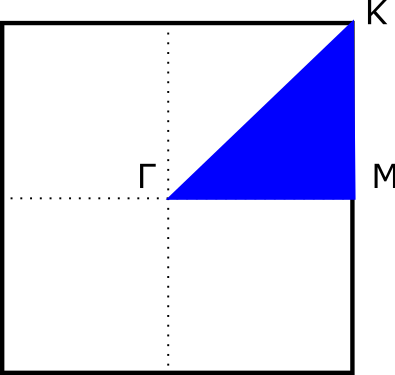
\includegraphics[width=0.3\textwidth]{imgs/sqibz.png}
\caption{\label{fig:ibzonesq} The irreducible Brillouin zone of the 2d square
    lattice in reciprocal space (blue).}
\end{figure}

With these concepts, we can fully solve the dispersion relation over our
infinite lattice space by just finding the solutions within the irreducible
Brillouin zone. Even more, given that standing waves are only present on the
boundary of the irreducible Brillouin zone, we only need to solve the
dispersion relation over the boundary.
%TODO: Is it because of standing waves??

Therefore for this case of an infinite 2d square lattice, we first solve the
eigen-problem we have in \eqref{eq:sqeig} over the boundary of the irreducible
Brillouin zone as shown in Figure~\ref{fig:ibzonesq}. We do this in Matlab by
varying the values of $\kappa_{x}$ and $\kappa_{y}$ which correspond to the
locus of points on the boundary of the irreducible Brillouin zone, and then
solve the eigen-problem for the eigenvalues and eigenvectors, which represent
$\matr{Omega}$ and $\vec{y}$ respectively. Then, we get the dispersion relation
by plotting out $\Omega_i$ against $(\kappa_x,\kappa_y$ or the position on the
Brillouin zone.

\textit{Note}: The significance of the eigenvectors or $y_i$ will be discussed
more in Chapter \ref{}.
%TODO: Do we need to use the eigenvectors?

We first need to find the values of $\kappa_{x}$ and $\kappa_{y}$ at $\Gamma$,
$X$ and $M$ as shown in Figure~\ref{fig:ibzonesq}.
%TODO: What should the limits of kappa_x and kappa_y be?

With this, and assuming that all masses $M_i=1$ for now (we will explore how
different perturbations in the lattice affect the dispersion relation in
Chapter \ref{perturbed}), we get the dispersion relation in
Figure~\ref{fig:sqdisper}. 
%TODO: Plot dispersion relation of 2d square lattice and explain?

\section{2d hexagonal lattice}
We will now consider how waves propagate across a 2d lattice made of hexagonal
elementary cells. 

\begin{figure}[!h]
\centering
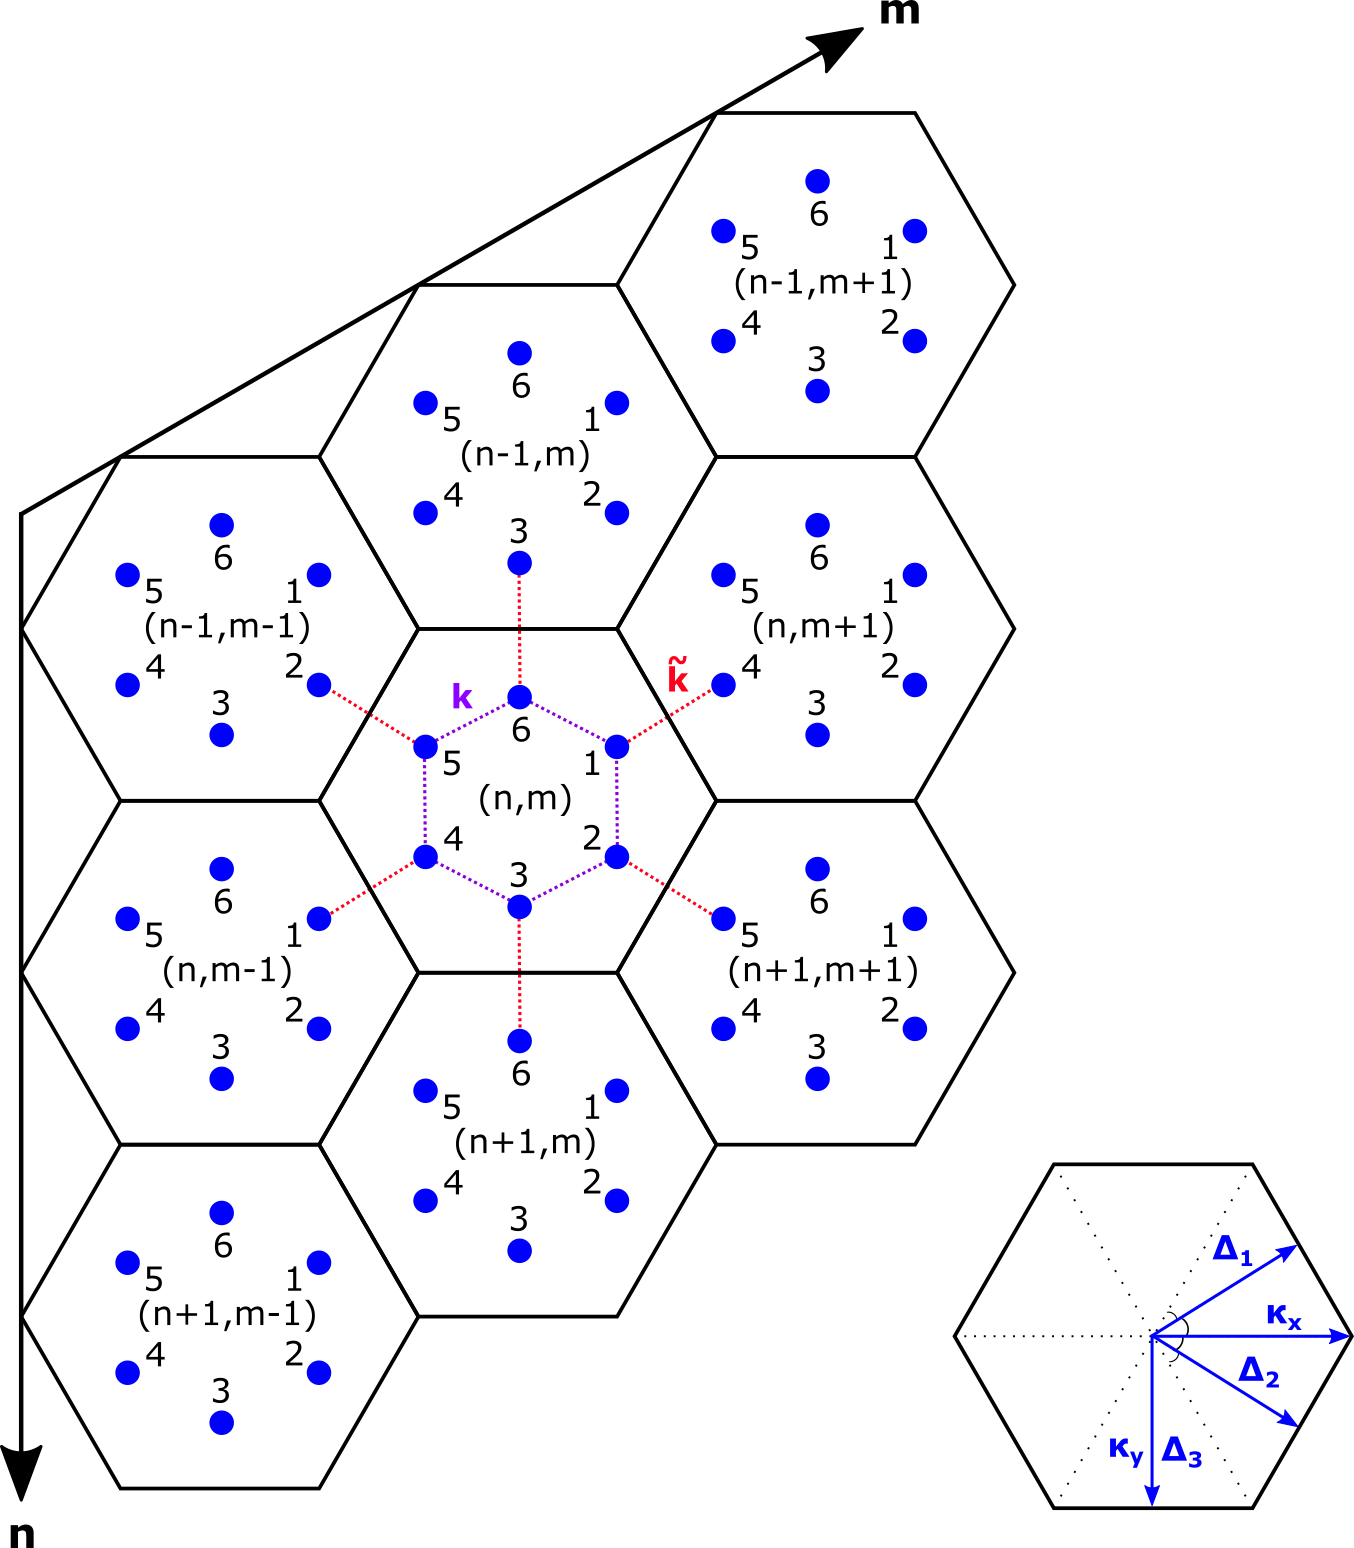
\includegraphics[width=0.8\textwidth]{imgs/hexmodel.png}
\caption{\label{fig:hexscheme} Schematic view of our 2d hexagonal model. Each
  hexagonal tile in the grid corresponds to one elementary cell with six
  masses. $k$ and $\tilde{k}$ represent the intra- and inter-cell spring
  constants respectively. The cell in the far bottom right shows the directions
  of the Bloch phases. Note that only the elastic interactions involving the
  masses in cell $(n,m)$ are shown to avoid cluttering the figure, although
  they exist within and between each cell.}
\end{figure}
%TODO: Check if this figure actually corresponds to our hex model. Source says it's for a triangular model

As described in Figure~\ref{fig:hexscheme}, consider an infinite 2d plane made
of hexagonal unit cells of six masses $M_i$ for $i\in\left[1,6\right]$, which
are arranged in an inner hexagon rotated $\frac{\pi}{6}$ relative to each cell.

Similarly to the 2d square lattice, we again consider only nearest neighbour
interactions and focus on the elementary cell $(n,m)$ and its adjacent cells.
Using Hooke's law and Newton's 2nd law on each of the masses in cell $(n,m)$,
we can get a second order differential equation which is coupled to the
displacements of the other masses it is connected to. For example, considering
$M_1^{n,m}$, we get

\begin{align}
  F_1=M_1\frac{d^{2}}{dt^{2}}y_1^{n,m}
      =k\left(y_2^{n,m}+y_6^{n,m}-2y_1^{n,m}\right)+
       \tilde{k}\left(y_4^{n,m+1}-y_1^{n,m}\right)
\label{eq:2dH1}
\end{align}

Now again we can use the periodicity of the lattice and Bloch's theorem to
relate the displacements of any mass to the displacement of the corresponding
mass in a \textit{base cell} using the lattice vectors shown in
Figure~\ref{fig:hexscheme}:

\begin{equation}
  \Delta_1=\sqrt{3}\kappa_x+\kappa_y
\label{eq:hexvec1}
\end{equation}

\begin{equation}
  \Delta_2=\sqrt{3}\kappa_x-\kappa_y
\label{eq:hexvec2}
\end{equation}

\begin{equation}
  \Delta_3=-2\kappa_y
\label{eq:hexvec3}
\end{equation}

With these, we can write out the relationship between the displacements for
neighbouring cells, e.g. for cell $(n,m)$ and its six nearest neighbours we
have

\begin{equation}
  y_4^{n,m+1}=e^{i\Delta_1}y_4^{n,m}
\label{eq:hexrelate4}
\end{equation}

\begin{equation}
  y_5^{n+1,m+1}=e^{i\Delta_2}y_5^{n,m}
\label{eq:hexrelate5}
\end{equation}

\begin{equation}
  y_6^{n+1,m}=e^{-i\Delta_3}y_6^{n,m}
\label{eq:hexrelate6}
\end{equation}

\begin{equation}
  y_1^{n,m-1}=e^{-i\Delta_1}y_1^{n,m}
\label{eq:hexrelate1}
\end{equation}

\begin{equation}
  y_2^{n-1,m-1}=e^{-i\Delta_2}y_2^{n,m}
\label{eq:hexrelate2}
\end{equation}

\begin{equation}
  y_3^{n-1,m}=e^{i\Delta_3}y_3^{n,m}
\label{eq:hexrelate3}
\end{equation}

Using these, dropping the superscripts and again assuming we have a Bloch wave
solution as described in \eqref{eq:wavesol}, \eqref{eq:2dH1} can be rewritten as 

\begin{align}
M_1\Omega_1^{2}y_1
      &=\left(2k+\tilde{k}\right)y_1-ky_2-\tilde{k}e^{i\Delta_1}y_4-ky_6
\label{eq:2dH2}
\end{align}

Similarly to the 2d square model case, we can construct this equation for each
$y_i$ and then reformulate the six difference equations as an eigen-problem

\begin{align}
  \left[\matr{A}\left(\kappa_{x},\kappa_{y}\right)-\matr{\Omega}\matr{M}\right]\vec{y}=\vec{0}
\label{eq:hexeig}
\end{align}

where $\matr{\Omega}=\diag\left(\left\{\Omega_i^2\right\}\right)$,
$\matr{M}=\diag\left(\left\{M_i\right\}\right)$,
$\vec{y}=\left[\left\{y_i\right\}\right]^T$ and now

\begin{align}
  \matr{A}\left(\kappa_{x},\kappa_{y}\right)=\left[
\begin{array}{cccccc}
2k+\tilde{k} & -k & 0 & -\tilde{k}e^{i\Delta_1} & 0 & -k\\
-k & 2k+\tilde{k} & -k & 0 & -\tilde{k}e^{i\Delta_2} & 0\\
0 & -k & 2k +\tilde{k} & -k & 0 & -\tilde{k}e^{-i\Delta_3}\\
-\tilde{k}e^{-i\Delta_1} & 0 & -k & 2k+\tilde{k} & -k & 0\\
0 & -\tilde{k}e^{-i\Delta_2} & 0 & -k & 2k+\tilde{k} & -k\\
-k & 0 & -\tilde{k}e^{i\Delta_3} & 0 & -k & 2k+\tilde{k}
\end{array}\right]
\end{align}

We will again use the theory of Brillouin zones as described in Chapter
\ref{brizones} to simplify the work we need to do in order to understand the
dispersion relation of this 2d hexagonal lattice.

\begin{figure}[!h]
\centering
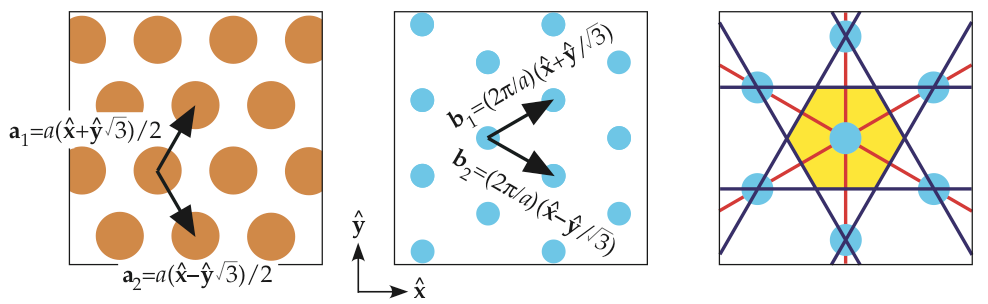
\includegraphics[width=0.8\textwidth]{imgs/bzonehex.png}
\caption{\label{fig:bzonehex} On the left is the lattice points in real space.
    In the middle is the corresponding reciprocal lattice. On the right is the
    construction of the first Brillouin zone: straight lines are drawn from the
    origin to the other lattice points (red), their perpendicular bisectors are
    the Bragg planes (blue), and the innermost region enclosed by the Bragg
    planes is the first Brilloin zone (yellow). Image and caption adapted from
    source.\cite{MITnp}}
\end{figure}
%TODO: Explain image equations?

\begin{figure}[!h]
\centering
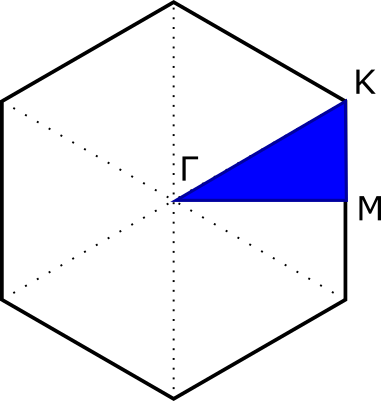
\includegraphics[width=0.3\textwidth]{imgs/hexibz.png}
\caption{\label{fig:ibzonehex} The irreducible Brillouin zone of the 2d
    hexagonal lattice in reciprocal space (blue).}
\end{figure}

Now as before, we can solve the dispersion relation over our infinite lattice
by just solving it over the boundary of the irreducible Brillouin as shown in
Figure~\ref{fig:ibzonehex}. First, let us find the values of $\kappa_{x}$ and
$\kappa_{y}$ at $\Gamma$, $K$ and $M$ as shown in the figure. We take
$\Gamma=(0,0)$ since it is the origin. 
%TODO: How to get K and M?

With this, and taking $M_i=k=\tilde{k}=1$ for simplicity, we get the dispersion
relation in Figure~\ref{fig:hexdisper}.

\begin{figure}[!h]
\centering
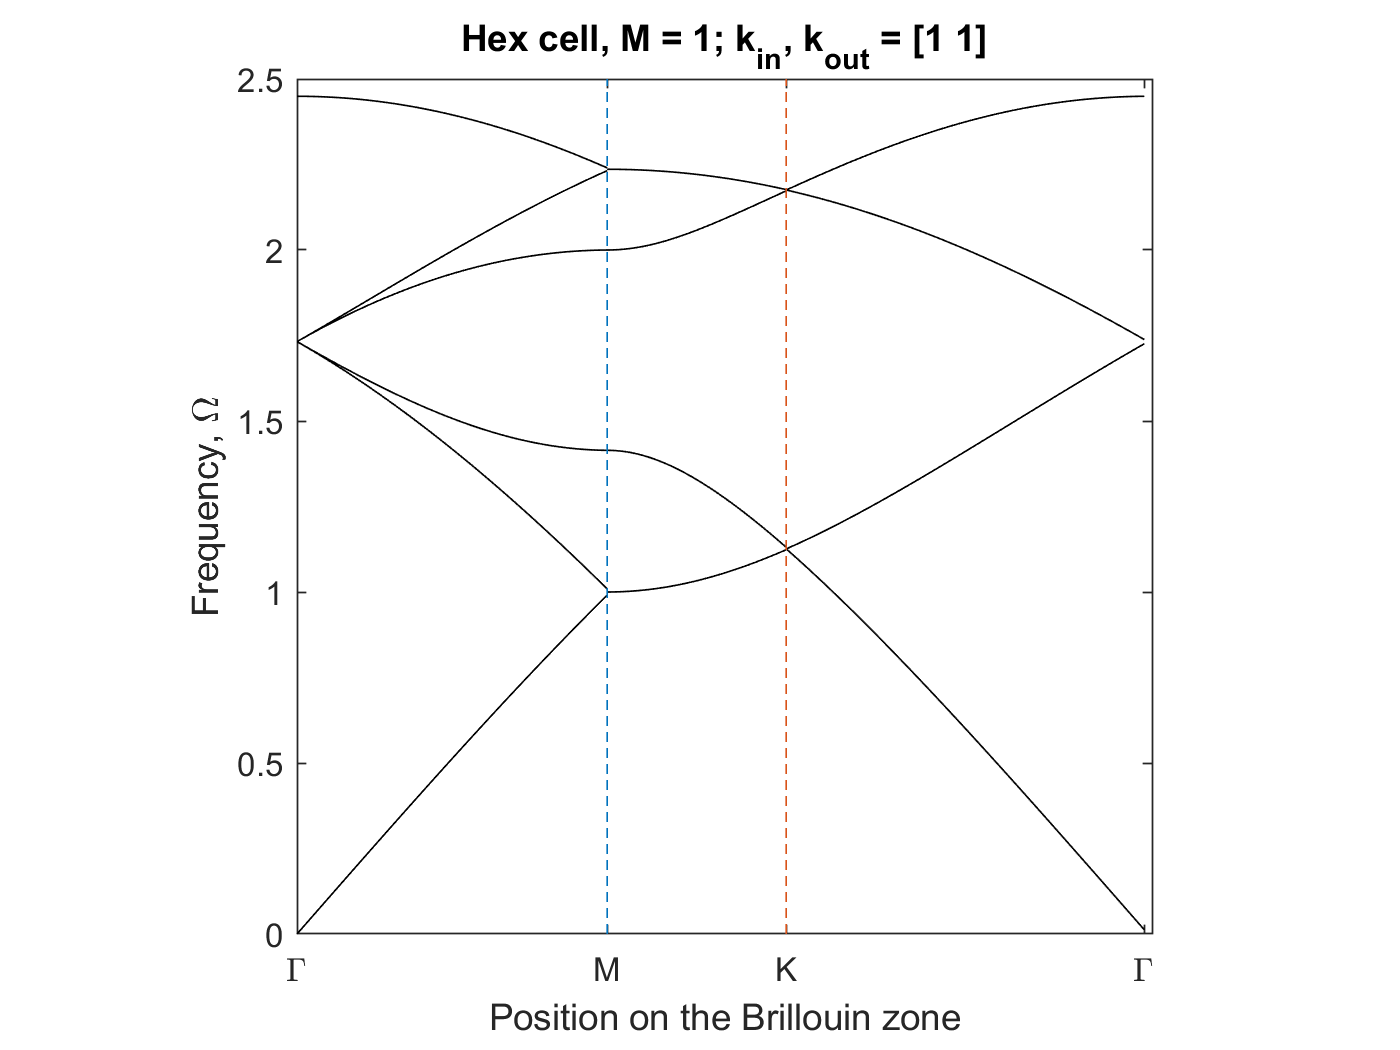
\includegraphics[width=0.8\textwidth]{imgs/hexdisper.png}
\caption{\label{fig:hexdisper} The dispersion relation of the 2d hexagonal
    lattice with $M_i=k=\tilde{k}=1$.}
\end{figure}

%TODO: Complete discussion of hex dispersion relation

\section{2d kagome lattice}
We will now investigate the kagome lattice, which is also known as the
trihexagonal tiling as it consists of triangles surrounding hexagons, as shown
in Figure~\ref{fig:kagomescheme}.

\begin{figure}[!h]
\centering
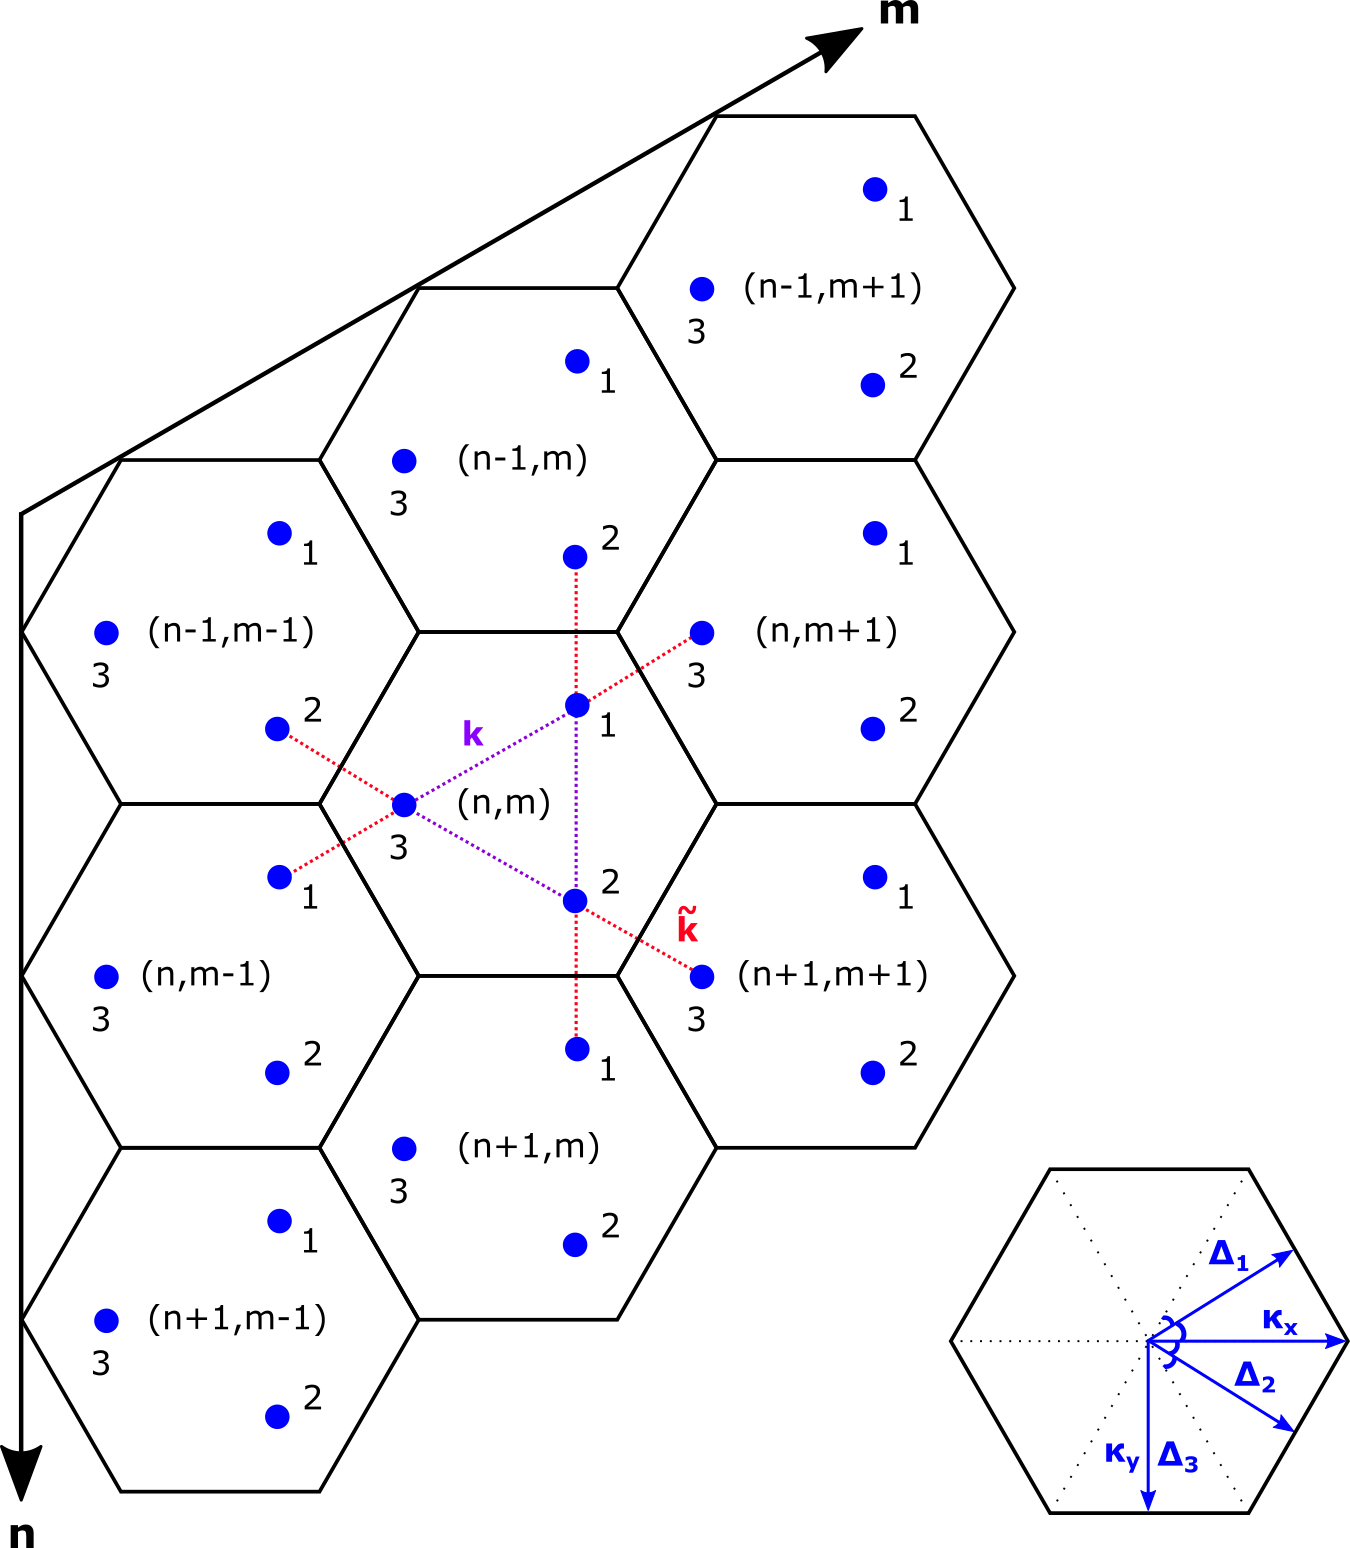
\includegraphics[width=0.8\textwidth]{imgs/kagomemodel.png}
\caption{\label{fig:kagomescheme} Schematic view of our 2d kagome model. Each
  hexagonal tile in the grid corresponds to one elementary cell with three
  masses. $k$ and $\tilde{k}$ represent the intra- and inter-cell spring
  constants respectively. The cell in the far bottom right shows the directions
  of the Bloch phases. Note that only the elastic interactions involving the
  masses in cell $(n,m)$ are shown to avoid cluttering the figure, although
  they exist within and between each cell.}
\end{figure}

Now again playing the same game as before, we can construct second order
differential equations which couple the displacements of connected masses. For
example, considering $M_1^{n,m}$, we get

\begin{align}
  F_1=M_1\frac{d^{2}}{dt^{2}}y_1^{n,m}
      =k\left(y_2^{n,m}+y_3^{n,m}-2y_1^{n,m}\right)+
       \tilde{k}\left(y_2^{n-1,m}+y_3^{n,m+1}-2y_1^{n,m}\right)
\label{eq:2dK1}
\end{align}

Due to the similarities in the shape of the elementary cell of the kagome
lattice and the hexagonal lattice, the Bloch phases are the same and we can
reuse \eqref{eq:hexvec1}, \eqref{eq:hexvec2} and \eqref{eq:hexvec3} as lattice
vectors. In doing so, we find the following relationships:

\begin{equation}
  y_1^{n+1,m}=e^{i\Delta_3}y_1^{n,m}
\label{eq:kagomerelate1a}
\end{equation}

\begin{equation}
  y_1^{n,m-1}=e^{-i\Delta_1}y_1^{n,m}
\label{eq:kagomerelate1b}
\end{equation}

\begin{equation}
  y_2^{n-1,m}=e^{-i\Delta_3}y_2^{n,m}
\label{eq:kagomerelate2a}
\end{equation}

\begin{equation}
  y_2^{n-1,m-1}=e^{-i\Delta_2}y_2^{n,m}
\label{eq:kagomerelate2b}
\end{equation}

\begin{equation}
  y_3^{n,m+1}=e^{i\Delta_1}y_3^{n,m}
\label{eq:kagomerelate3a}
\end{equation}

\begin{equation}
  y_3^{n+1,m+1}=e^{i\Delta_2}y_3^{n,m}
\label{eq:kagomerelate3b}
\end{equation}

With these, and assuming we have a Bloch wave solution as described in
\eqref{eq:wavesol}, we can rewrite \eqref{eq:2dK1} as

\begin{align}
M_1\Omega_1^{2}y_1
      &=\left(2k+2\tilde{k}\right)y_1+\left(-k-\tilde{k}e^{-i\Delta_3}\right)y_2+\left(-k-\tilde{k}e^{i\Delta_1}\right)y_3
\label{eq:2dK2}
\end{align}

Again, by forming these equations for each of the three masses, and then
combining them into one matrix equation, we get the following eigen-problem.

\begin{align}
  \left[\matr{A}\left(\kappa_{x},\kappa_{y}\right)-\matr{\Omega}\matr{M}\right]\vec{y}=\vec{0}
\label{eq:kagomeeig}
\end{align}

where $\matr{\Omega}=\diag\left(\left\{\Omega_i^2\right\}\right)$,
$\matr{M}=\diag\left(\left\{M_i\right\}\right)$,
$\vec{y}=\left[\left\{y_i\right\}\right]^T$ and now

\begin{align}
  \matr{A}\left(\kappa_{x},\kappa_{y}\right)=\left[
\begin{array}{ccc}
2k+2\tilde{k} & -k-\tilde{k}e^{-i\Delta_3} & -k-\tilde{k}e^{i\Delta_1} \\
-k-\tilde{k}e^{i\Delta_3} & 2k+2\tilde{k} & -k-\tilde{k}e^{i\Delta_2} \\
-k-\tilde{k}e^{-i\Delta_1} & -k-\tilde{k}e^{-i\Delta_2} & 2k+2\tilde{k} 
\end{array}\right]
\end{align}

%TODO: Form equations up till eigenproblem

Again given the similarities between the kagome and hexagonal lattice, the
irreducible Brillouin zones happen to be identical as seen in
Figure~\ref{fig:ibzonekagome}.

\begin{figure}[!h]
\centering
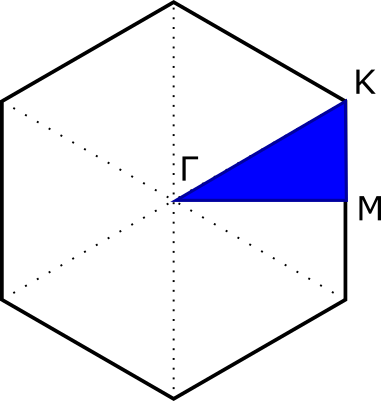
\includegraphics[width=0.3\textwidth]{imgs/kagomeibz.png}
\caption{\label{fig:ibzonekagome} The irreducible Brillouin zone of the 2d
    kagome lattice in reciprocal space (blue).}
\end{figure}

By solving this eigen-problem along the boundaries of the irreducible Brillouin
zone shown, we get the dispersion relation in Figure~\ref{fig:kagomedisper}.

\begin{figure}[!h]
\centering
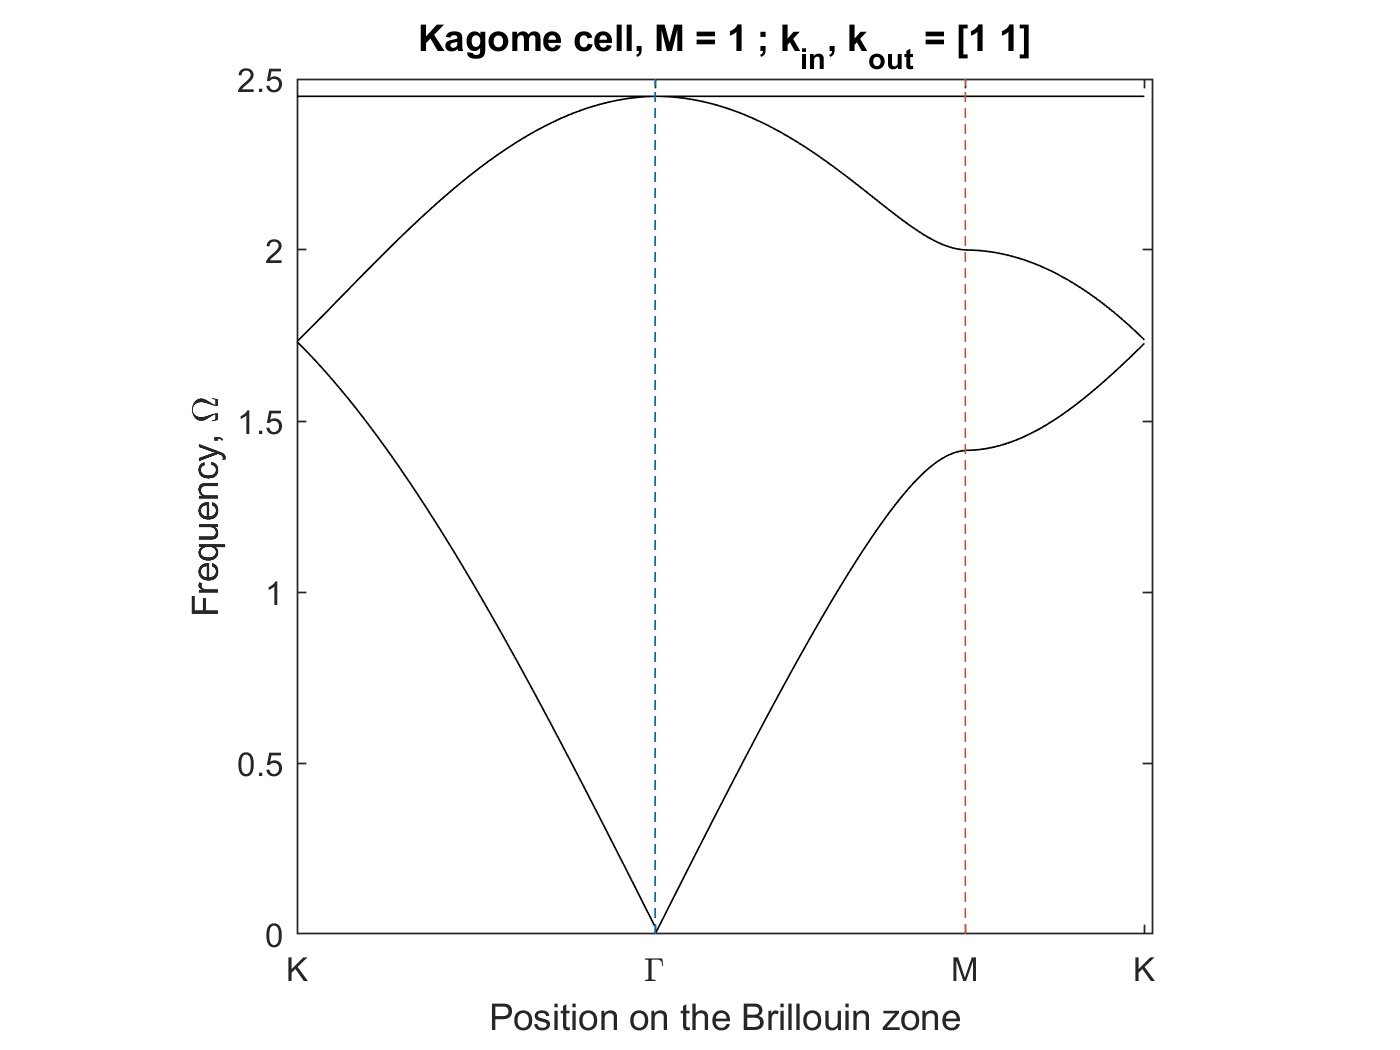
\includegraphics[width=0.8\textwidth]{imgs/kagomedisper.png}
\caption{\label{fig:kagomedisper} The dispersion relation of the 2d kagome
    lattice with $M_i=k=\tilde{k}=1$.}
\end{figure}

What is really interesting about this dispersion relation is that there is one
eigenvalue solution which is constant over the boundary of the irreducible
Brillouin zone; but not only that, it is actually constant over the entire
space!
%TODO: Explain why there is a flat line in kagome dispersion relation
%TODO: Explain significance of dispersion relation
